\documentclass[../main.tex]{subfiles}
\begin{document}

In this chapter, we describe the project's design principles,
including its architectural foundation.

\section{Function as a Service}\label{sec:FaaS}

We define FaaS platforms as an environment to run a set of programmable and stateless functions,
which are reachable from inside or the outside through invocation. 
The main difference to ordinary PaaS platforms is abstraction from a server centered model: 
A developer can develop and deploy a function without needing to know about a server, hence the common name serverless. 
An invocation can happen through so-called triggers which can be defined on events 
such as an incoming HTTP request or an event from another program such as creating a file in an S3 bucket. 
The common entry point and interface to every function deployed to such a FaaS platform is the HTTP protocol 
over which parameters and their responses are serialized. 
We call a set of related FaaS functions a program. A simple such program setup is illustrated in \Cref{fig:frameworkSimpleProgramSetup}

\begin{figure}
\begin{center}
  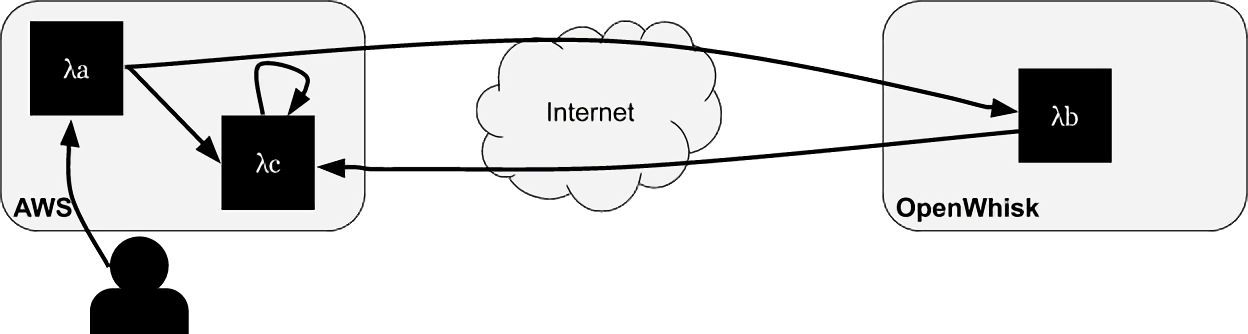
\includegraphics[width=\linewidth,keepaspectratio]{./3-functions.png}
\end{center}
\caption[Simple FaaS Program Setup]{A simple FaaS program setup consisting of three functions which are deployed on two platforms (AWS and Openwhisk). 
They generally communicate via the internet (HTPP).}%
\label{fig:frameworkSimpleProgramSetup}
\end{figure}

\subsection{FaaS Function Language}%
\label{sub:FaaSLanguage}

When FaaS was first introduced into the public by AWS in 2014, Node.js (JavaScript) was the only supported target%
\footnote{\url{https://docs.aws.amazon.com/lambda/latest/dg/lambda-releases.html}}. 
Later more cloud platforms and frameworks also adopted the FaaS principle, 
where a majority have also started with Node.js as their first target language. 
At the time of this writing more languages than Node.js were introduced such as Python or Golang. 
Nevertheless, Node.js has been the established language ever since the first AWS lambda release.

Thus, the majority of FaaS platforms support Node.js as only or first target. 
We intend to target this language in our further design and benchmarking library 
in order to be language compatible with the majority of FaaS platforms.

\subsection{FaaS Call Graph}%
\label{sub:FaaSCallGraph}

Each program can be represented as a directed graph, 
with each node serving a function instance and each vertex a call to a function (\Cref{fig:frameworkSimpleProgramCallGraph}). 
It is possible to have a reflexive or cyclic graph in case of recursion. 
Each deployed function usually has only one endpoint, 
meaning that we do not route into multiple HTTP subpaths within a function.

\begin{figure}
\begin{center}
  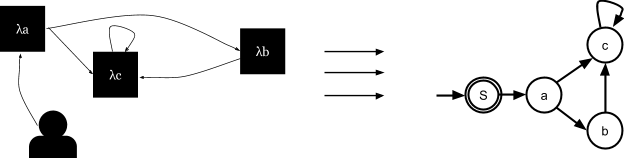
\includegraphics[width=\linewidth,keepaspectratio]{./simple-call-graph.png}
\end{center}
\caption[A FaaS Program's Call Graph]{A simple FaaS program, together with its call graph.}%
\label{fig:frameworkSimpleProgramCallGraph}
\end{figure}

\section{Benchmarking Framework}\label{sec:Framework}

With this work, we introduce a comprehensive framework for running experiments 
to generate tests and benchmark data of complex FaaS programs that are hosted on and communicate between different FaaS providers. 
The framework should make it possible to easily create more complex FaaS based applications which can also be benchmarked 
across a set of different providers.

We further want to make extension to novel providers by other researchers as convenient as possible. 
Thus we are trying to keep the required amount of needed interfaces to providers small 
such that it is possible to evaluate early-stage prototypes with our framework. 
As we cannot expect all platforms to provide measurement capabilities, 
we change the deployed program with our framework to compile measurement capabilities into the deployed code 
such that the program is measuring itself. 
This approach is called instrumentation and is further discussed in \Cref{sec:instrumentationCapabilities}.

Additionally, we have extended the framework to make the setup and deployment of a program on multiple platforms automated. 
This automatic setup is also responsible for compiling a program and configuring our instrumentation-library, 
which offers a high-level interface to researchers for measuring their deployed program. 
Finally it automates the deployment of these programs and the benchmarking and extracting of data 
to offer a one-stop shop comprehensive solution for multi-platform benchmarking.

\subsubsection{Components}%
\label{sub:frameworkComponents}

The framework is split into three subprojects, maintained as git repositories under the FaaSterMetrics name%
\footnote{\url{https://github.com/FaaSterMetrics}}. 
We have an overarching ``experiments'' repository which serves as the main entry point to the project.
The ``lib'' repository contains our platform-agnostic instrumentation-library
and ``analysis'' is responsible for analyzing raw generated data from the program to extract meaningful data for further processing.  
This document is found in the ``documentation'' repository.


\section{Experiments}%
\label{sec:experiments}

In our context, any experiment consists of a deployed program and a workload running against this program.
The expectation we have from an experiment is to generate data that will be used to evaluate a platform. 
When the program or other factors of the experiment are changed, the experiment will be re-run.

We found that requirements that are needed for running a program in production and 
for analyzing a program for scientific purposes often differ. 
A program in production usually needs uptime and reliability as well as security. 
However, these aspects are mostly not relevant for experimentally benchmarking a platform and for generating scientific measurement data. 
We have decided to engineer and dedicate our framework to be used primarily for scientific purposes
and thus mostly disregard the production-specific requirements listed above.

The framework's design allows a pre-defined high-level workflow (\Cref{fig:experimentWorkflowDiagram}),
which we have found to be used throughout many different scientific environments 
and which is directed towards allowing simple experiment reproducibility.

\begin{figure}
\begin{center}
  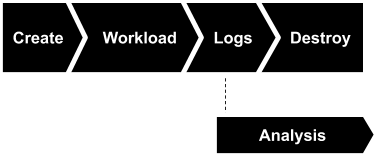
\includegraphics[width=\linewidth,keepaspectratio]{./workflow-diagram.png}
\end{center}
\caption{General Experiment Workflow Diagram}%
\label{fig:experimentWorkflowDiagram}
\end{figure}

The goal of each experiment is to generate data describing the program and the used platforms 
so that meaningful results can be extracted from the generated data. 
Also, all experiments and variables that result in produced data shall be easily controllable 
such that a reviewer can reproduce and verify data and results.
Specifically, an experiment consists of a program and the workload executed against this program. 
Thus the program as well as the workload need to be described such that resulting data can be reproduced.

As shown in \Cref{fig:experimentWorkflowDiagram}, our experiments follow certain workflow steps: 
\begin{enumerate}
  \item The program is generated and deployed from a local file representation.
  \item The experiment workload generator is deployed and executed.
  \item All logs are collected and locally aggregated.
  \item Finally, the deployed experiment gets destroyed and the downloaded logs can be analyzed.
\end{enumerate}
In \Cref{chap:analysis} we introduce our analysis tools, which are responsible for 
extracting data from the logs and further to produce measurement results from the extracted data.
The workload generation and its parameters are discussed in TODO oof.

\subsection{Experiment Configuration}\label{sec:experimentConfig}

An experiment is defined by a program and its services. 
In this section, we discuss how to make an experiment reproducible. 

To limit changes between experiments, the program and optionally a database shall be deployed in the same way on the same platforms, 
and the workload executed onto the program shall be the same. 
Thus, the kind of workload and all information about which deployment configuration
to use per function in a program within an experiment is declared in an experiment.json config file.

\begin{figure}
  \begin{tcolorbox}
    \begin{minted}[autogobble]{json}
    {
      "services": {
        "redis": {},
        "workload": {
          "config": "./workload.yml"
        }
      },
      "program": {
        "frontend": {
          "provider": "aws",
          "calls": ["currency"]
        },
        "currency": {
          "provider": "google"
        }
      }
    }
    \end{minted}
  \end{tcolorbox}
\caption[experiment.json Config Example]{An example \texttt{experiment.json} file. 
Therein, we have two functions: \texttt{frontend} and \texttt{currency}. The former calls the latter.}%
\label{fig:exampleExperimentConfig}
\end{figure}

An example of an \texttt{experiment.json} is shown in \Cref{fig:exampleExperimentConfig}.
The~.json as file extension already indicates a JSON structured text file which follows a specific scheme. 
The general hierarchy is split between service and program definition.

The program is  composed of the set of functions with the name as their key in the first level, 
this ensures the uniqueness of the function names. 
Each function carries a provider and potentially configuration overwrites so that the deployment provider can decide 
on which platform to put a function. 
Each function also states their callee functions they intend to invoke during execution in the \mintinline{json}{"calls"} field. 
In case of recursion the function shall list itself. 

\subsection{Experiment Directory Structure}%
\label{sec:experimentDirectoryStructure}

\Cref{fig:experimentDirTree} shows the experiment directory structure.
In the experiment's main directory, one can see the functions folder which defines the different function names and their target JS files. 
The benchmarking framework is opinionated in the sense that a specific folder structure is expected. 
In the root the \texttt{experiment.json} file is mapping provider configurations to each function. 
The functions each lie in separate directories, each in their respective \texttt{/functions/<common-function-name>} directory.

\begin{figure}
\begin{tcolorbox}
\dirtree{%
.1 experiments.
.2 <experiment\_name>.
.3 experiment.json <- describes program and services.
.3 functions.
.4 <function\_1>.
.5 index.js.
.4 <function\_2>.
.5 index.js.
.5 <optional\_auxiliary\_file>.
}
\end{tcolorbox}
\caption[Typical Experiment Directory Structure.]{%
  A typical experiment directory structure. The \texttt{experiment.json} config file lies in the particular experiment's main directory.
  Within the \texttt{functions} subdirectory all functions have their own folders. 
  Each of them must contain an \texttt{index.js} file (with Node.js module semantics, see \Cref{sub:functionNaming} for usage),
  but they may of course use more files.
}%
\label{fig:experimentDirTree}
\end{figure}

\subsection{Terraform as FaaS \& Cloud Provider Abstraction}%
\label{sec:terraform}

When running an experiment, we need to be able to deploy the functions, aggregate generated logs, and tear everything down. 
Anything which can fulfill these requirements could be used to run an experiment.

For our chosen FaaS providers, the deployment and configuration of the platforms are managed with the Infrastructure as Code tool terraform%
\footnote{\url{https://www.terraform.io}}. 
It enables us to create reproducible test setups for all major cloud platform providers and to extend it to novel providers. 
Since terraform allows abstraction and parameterization we 
leverage terraforms capabilities when interacting with cloud providers and FaaS platforms as much as possible.
This means that terraform is mainly internally responsible for deploying and destroying our programs.
We also successfully extended terraform to support novel platforms, e.g.\@ MCC's tinyFaaS platform.

% Well, this is dirty.
\subfile{../experimentStructure/workloads.tex}

\section{Function Wrapper Library}%
\label{sec:designFunctionWrapper}

True to the standard FaaS paradigm, we intend to have single call functions only. 
This way, we can define a single endpoint for each deployed function and use its unique function name globally 
(even across different platforms), also see Section ``Definition of Experiments''. 
This enables us to easily define our own small RPC framework, as shown below.

\subsection{Function Handler}%
\label{sub:designFunctionHandler}

Since each platform comes with its own function implementation and way to define function prototypes, 
we abstract away the different interfaces into a new unified one. 
To this end, a library-provided function wrapper, called `RPC handler' is used.

This approach then makes it possible to move functions from one provider to another, 
assuming no platform specific APIs have been used within the function (which we avoid). 
Some platform-specific behavior also has to be mocked for compatibility, 
e.g.\@ that GCP uses a different JSON body parsing as AWS.\@

Our RPC handler accepts a JSON body from the HTTP request and returns a JSON object. 
This convention makes it possible to implement straight forward (natural looking) JavaScript functions. 
Usage instructions about this handler can be found in \Cref{ssub:rpcHandler}.

\subsection{Function Call (Stub)}%
\label{sub:designFunctionCalls}

\begin{figure}
\begin{center}
  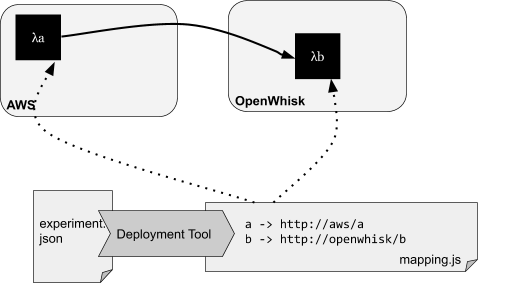
\includegraphics[width=\linewidth,keepaspectratio]{./deployment-tool.png}
\end{center}
\caption{Automatic Function Deployment}%
\label{fig:functionDeployment}
\end{figure}

Functions in our program need to be able to call each other, independent of where the functions are deployed. 
We have defined our function interface to be wrapped by an RPC framework, 
so we can utilize this further to abstract real function URLs to the canonical name of the function. 

The framework has to be able to map the canonical name to the real function URL, 
as we want to abstract the peer URL so that the caller code is agnostic to where the callee is deployed. 
As the URL of a function is deployment specific and only known by the deployment tool, 
it is thus possible to compile all endpoint mappings into the source code. 
When using the RPC stub, we map the function name against the created route of the RPC receiver. 
All of the function to URL mappings are created from the \texttt{experiment.json} in combination with the deployment tool
(\Cref{fig:functionDeployment}). 
The resulting \texttt{mapping.js} will be used to call the peer functions by its name so that developers
do not need to know about the actual URLs and can work with canonical names of the functions.

\subsection{Dependency Management}%
\label{sub:designLibsDeps}

Our function wrapping library naturally is a dependency for using the framework.
Moreover, with each new FaaS platform the number of external Node.js 
package dependencies increases.
This is why we include all necessary JS code into one file and inject it into the actual function files. 
This way all of our dependencies and business logic are bundled into a single deployable file. 
We use the ncc\footnote{\url{https://github.com/vercel/ncc}} project to achieve this.

\section{Function Logging}%
\label{sec:functionLogging}

The variety of FaaS platforms poses a challenge as there is no general interface and standardization to the deployed functions. 
The only standard interface exposed by every FaaS implementation is the HTTP serial interface. 
It would be beneficial to send the experiment measurements over this interface. 
However, we decided to not modify the request as this will modify the experiment as the transmission load/time 
would be changed due to the amount of information gathered in an experiment.
Instead, we use standard log output.

\subsection{FaaS Logging Assumptions}%
\label{sub:designLoggingAssumptions}

We have to send experiment measurements from the remote FaaS functions to the local experiment conductor. 
For this, we assume that every function has stdout logging as another interface exposed. 
Specifically we assume that after the experiment was conducted retrieval of logs from all platforms is possible. 
However, this makes it impossible to receive live experiment measurement data.

\subsection{FaaS Logging Overhead}%
\label{sub:designLoggingOverhead}

Before we decided to use logging output as a generalized interface to receive messages from multiple platforms, 
we wanted to determine the resulting overhead.
To estimate the impact and overhead of logging, we benchmarked AWS, Azure, and GCP printing performance. 

This way, we got an overview of how performance differs depending on the provider -- using the data gathered 
in the experiment; we later concluded that standard logging is a~viable option.
We tested log output of different sizes and different repetitions. 
For each test, we took 20 samples to avoid fluctuations.
We internally measured the runtime and return the time in the function response. 
The code to reproduce the experiments can be found in our GitHub ``test'' repository%
\footnote{\url{https://github.com/FaaSterMetrics/tests/blob/master/readme.md}}.

\subsection{FaaS Logging Verdict}%
\label{sub:designLoggingResult}

\begin{figure}
\begin{center}
  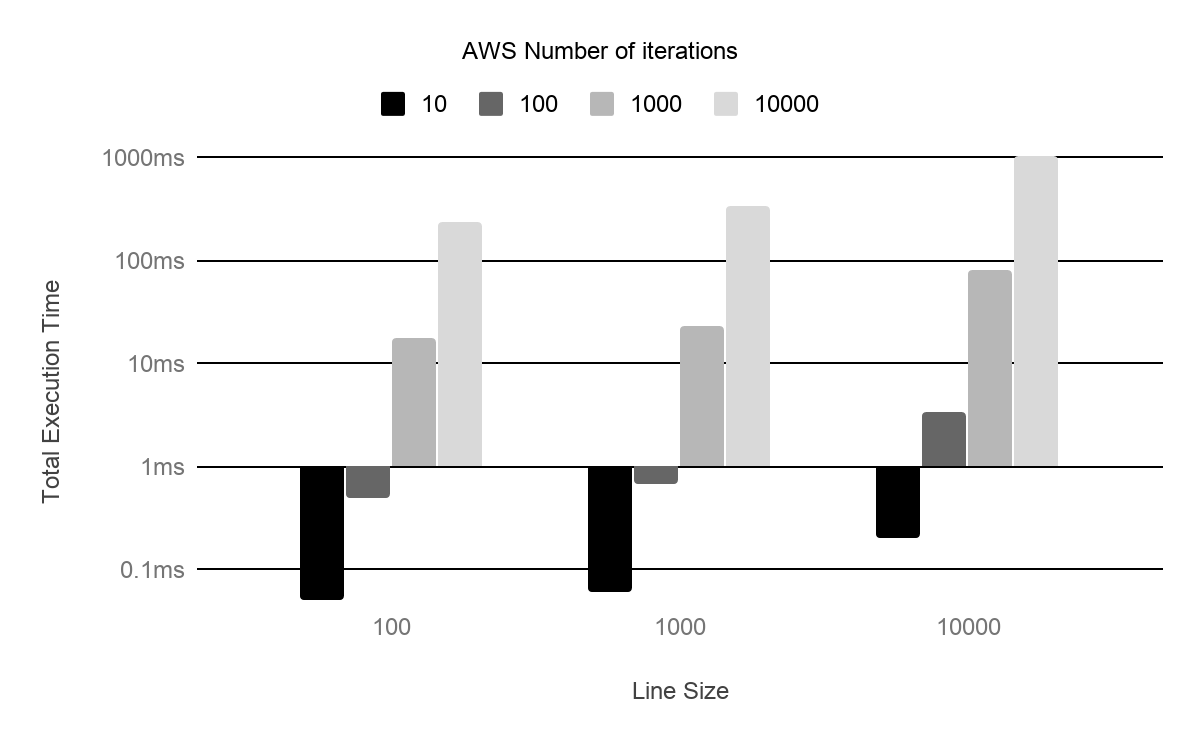
\includegraphics[width=11cm, keepaspectratio]{./AWS-logging.png}\\
  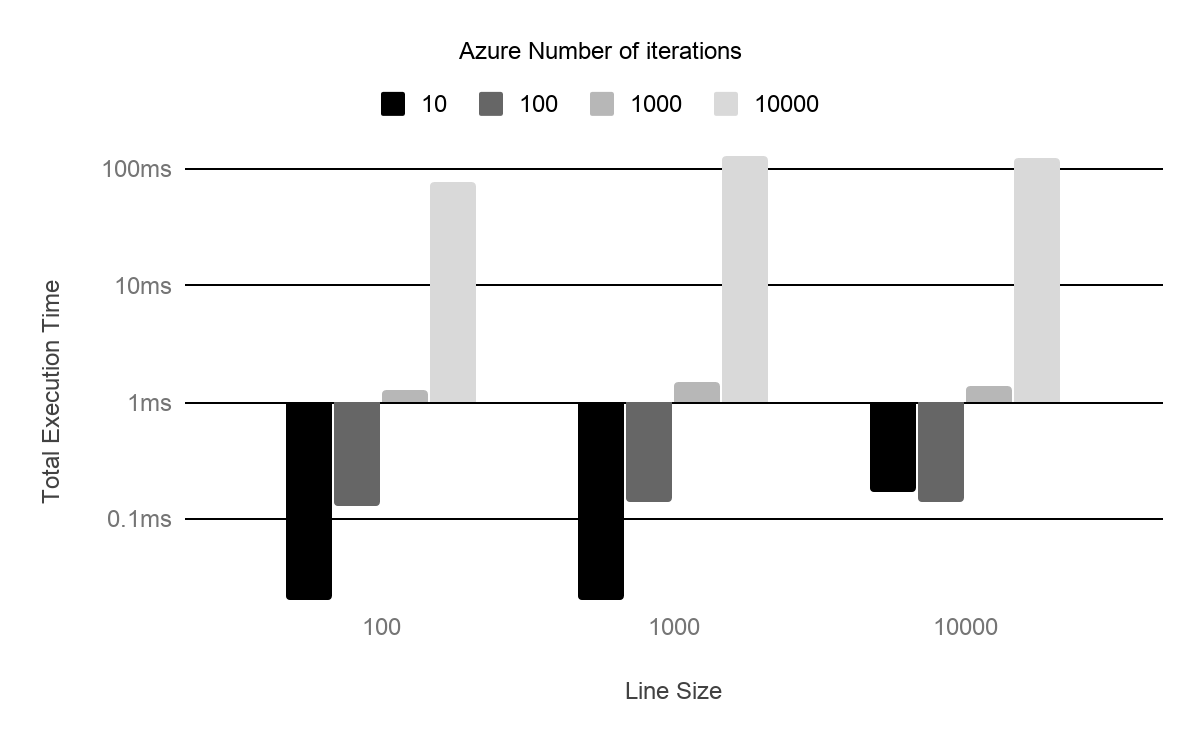
\includegraphics[width=11cm, keepaspectratio]{./Azure-logging.png}\\
  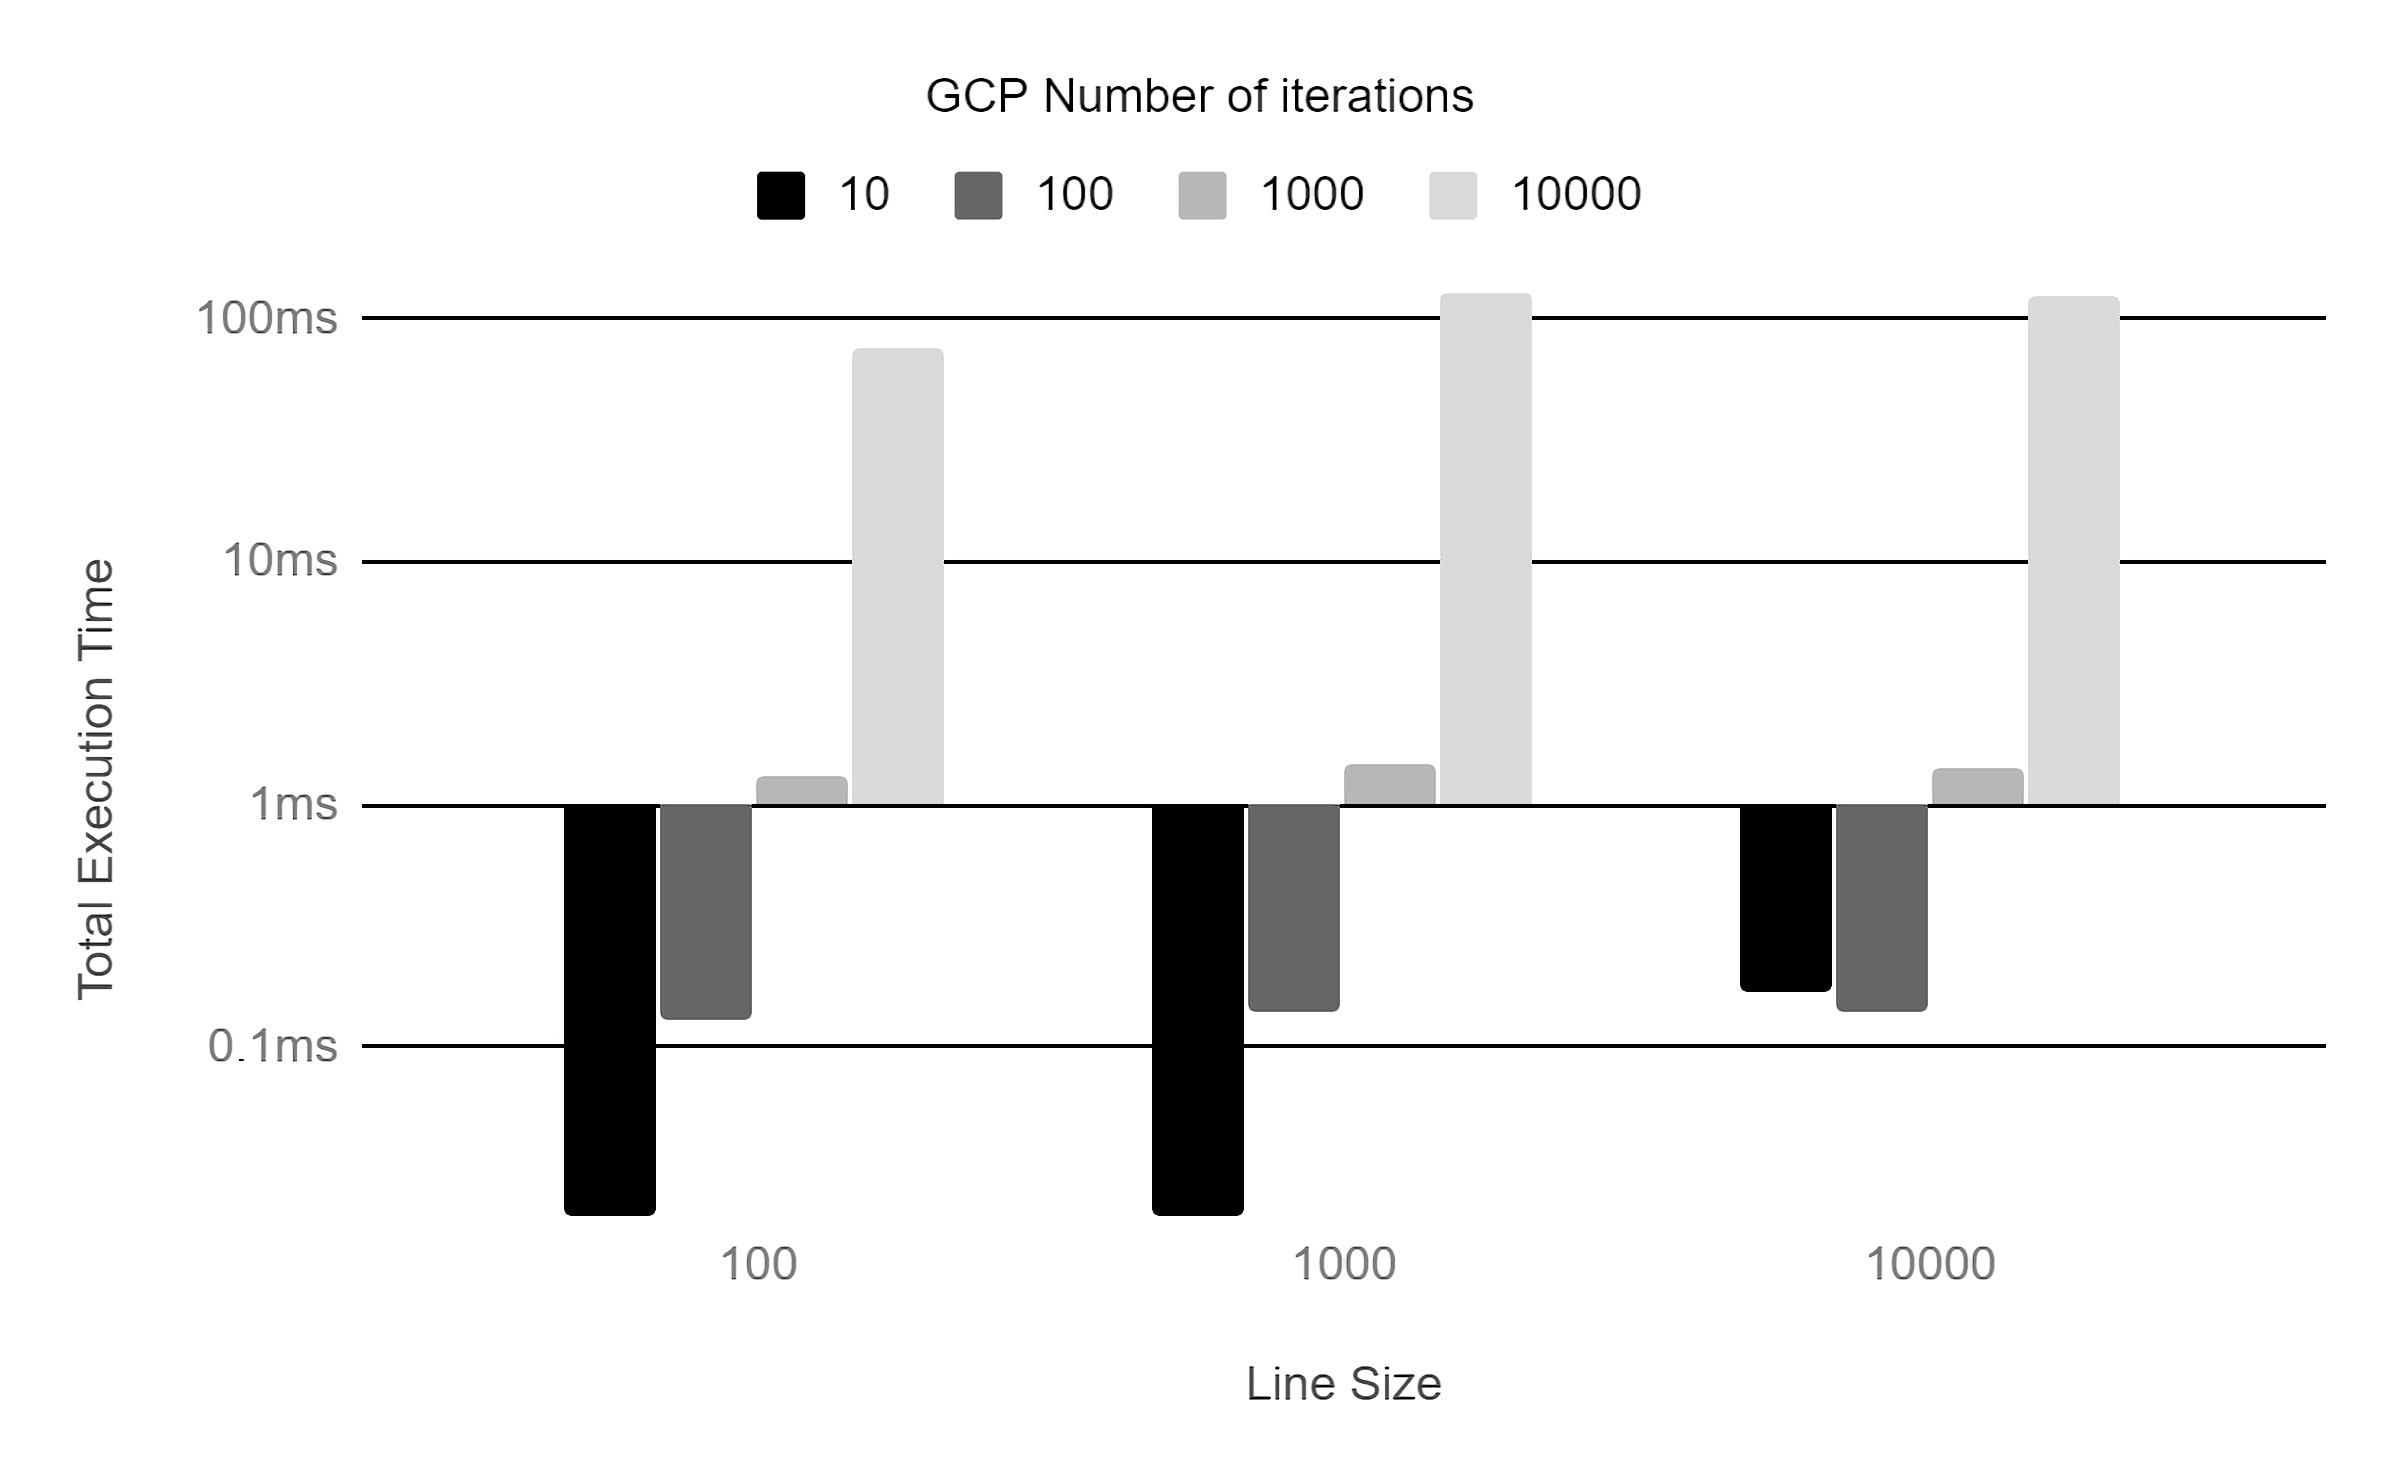
\includegraphics[width=11cm, keepaspectratio]{./GCP-logging.png}
\end{center}
\caption[Results of Logging Tests on AWS, GCP and Azure]{%
  We measured the time it took to print lines of 100, 1000, and 10000 characters to the console on three major FaaS providers. 
  The number of lines printed are increased from 10 to 10000 to get accurate results of how well a platform performs 
  under multiple logging statements which can occur during normal execution.
}
\label{fig:providerLoggingTest}
\end{figure}

For evaluating logging output performance, we considered overheads of up to 1ms as acceptable, 
since in more complex program setups we can have recursion and in general deep call trees which will be amplified by the logging overhead. 
Thus we do want to change the behaviour of a program by introducing arbitrary latency and 
overhead which can lead to different performance characteristics or even errors through timeouts.

Running the experiments showed us that we could observe two groups of requests behaving similarly. 
On all platforms, except for AWS, 
all log statements printed less than one thousand times were within our accepted interval, independent of the printed line size. 
When narrowing the criteria we can observe that AWS only fails on big logging statements which we deem acceptable.
Usually, we do not perform more than 10s of logging statements of a line size bigger than 10,000 characters anyway.

All in all, those results (shown in \Cref{fig:providerLoggingTest}) supported our thesis and we decided to let all functions log.



\section{Instrumentation Capabilities}%
\label{sec:instrumentationCapabilities}

In order to automatically measure our functions (and let them log), our library instruments its own code into those functions.
We define a single measurement as an event, these events will be dispatched to the log stream and later get aggregated. 
Each request in a program generates a set of measurable events from probes.

\subsection{Call tracing probes}%
\label{sub:callTracingProbes}

\begin{figure}
\begin{center}
  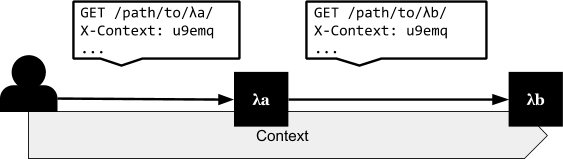
\includegraphics[width=\linewidth,keepaspectratio]{./multiple-functions-one-context.png}
\end{center}
\caption{Multiple Function Calls Under Same Context}%
\label{fig:contextID}
\end{figure}

We want to be able to analyze the temporal causality of a request in the program. 
To distinguish a request context, we introduce an $ O(1) $ sized request context token as shown in \Cref{fig:contextID}. 
This request token is unique and can later be used to group events together. 
As the token has constant size, we can include it in all network calls. 
Therefore, the (fairly low) overhead between different experiments will be the same, independent of the structure of the program.

When a function is called multiple times in a context, 
we need to be able to distinguish its calls in the temporal order. 
We assume that the system clocks are monotonic during the experiment interval, 
thus using the system time for each function to order the executions should be sufficient under a given context.

\subsubsection{Parallelism}%
\label{ssub:designFunctionParallelism}

\begin{figure}
\begin{center}
  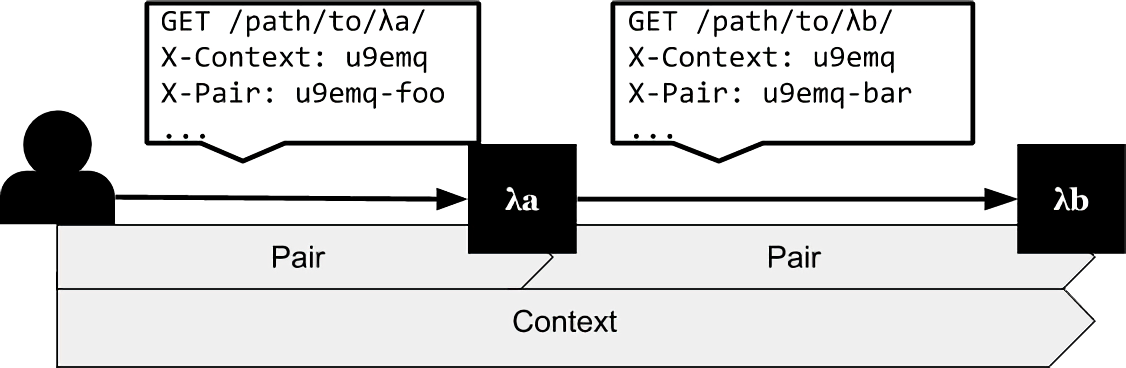
\includegraphics[width=\linewidth,keepaspectratio]{./multiple-functions-context-and-call-id.png}
\end{center}
\caption[Multiple Function Calls With Context and Pair IDs]{Same setup as \Cref{fig:contextID}, but also containing function pair IDs.}%
\label{fig:contextAndPairIDs}
\end{figure}

We cannot distinguish direct call connections on the same call invocation path under the same global context. 
As the call times are not serialized, we always add a direct call context which only lives from caller to callee and does not get propagated. 
Theoretically, we could constructs the global context from all call pairs. 
However for simplicity, we decided to include both IDs such that searching for a global context in pre-processing is much simpler.
An illustration is shown in \Cref{fig:contextAndPairIDs}.

\subsection{Runtime Probes}%
\label{sub:runtimeProbes}

\begin{figure}
  \begin{tcolorbox}
    \begin{minted}[autogobble]{js}
    exports.handler = async function(event, context) {
      measureFunctionTime("func:A", event, context, (e, c) -> {
        // real function code
      })
    }
    \end{minted}
  \end{tcolorbox}
\caption{Inserting Time Measurement to a Node.js Function}
\label{fig:timeMeasurementCode}
\end{figure}

To measure the actual runtime of any function we set time probes at the beginning and at the end of a function. 
Since function runtime data is fundamentally relevant for benchmarking, this probe should be present in every function.
Thus, our framewok always automatically injects appropriate measurement code into functions as shown
in \Cref{fig:timeMeasurementCode}. 

\subsection{Call Timing Probes}%
\label{sub:callingTimeProbes}

In our setting we measure real-world applications, which usually are represented by programs with multiple deep call hierarchies:
Functions are commonly invoking other functions or services such as a database. 
When calling another function or a service it is useful to know its runtime so that we can distinguish between runtime and network delay.

As long as we are calling into functions that use our framework, 
we can expect them to use our context and return their invocation time to us. 
However, when calling an external service, we cannot expect to get the time it took to process the request returned. 
Therefore, we have to distinguish between timing probes to functions or to external services.

\subsubsection{FaaS Function}%
\label{ssub:callingTimeProbeFunction}

\begin{figure}
\begin{center}
  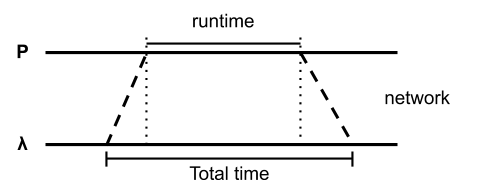
\includegraphics[]{./cristian.png}
\end{center}
\caption[Function Call Time Measurement]{%
  By applying Cristian's algorithm, we can determine the (averaged) network delay when calling 
  a FaaS function \textbf{P} from another function $\lambda$.
}
\label{fig:cristiansTimeMeasurement}
\end{figure}

When invoking another FaaS function we receive information about the actual runtime of the function.
Thus, we can use Cristian's algorithm \cite{cristian_probabilistic_1989} to calculate the network delay 
in addition to the runtime of the invoked function itself. 
This enables us to evaluate those network delays between functions (and usually providers). 
Also, we do not require both clocks to be synced perfectly, 
the only assumption is that they run approximately at the same speed in a small time frame (during invocation).

\subsubsection{External Services}%
\label{ssub:callingTimeProbeService}

\begin{figure}
\begin{center}
  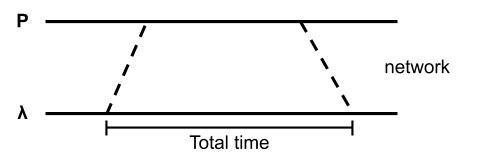
\includegraphics[]{./round-trip-time.png}
\end{center}
\caption[External Service Time Measurement]{%
  In contrast to \Cref{fig:cristiansTimeMeasurement}, we can not reason about the runtime of the called service \textbf{P} 
  from function $\lambda.$ Only the call's round-trip-time is known. 
  This~makes it impossible to isolate the network delay.
}
\label{fig:externalServiceTimeMeasurement}
\end{figure}

When measuring the invocation time to other services we can only extract the total round-trip time,
as we have no information about the actual running time of the program or of the time it takes the network to transmit the message.

\subsection{Coldstarts and Executors}%
\label{sub:coldStartProbing}

Even though serverless-FaaS platforms usually promise to offer development without caring about underlying hardware and to offer infinite scaling, 
a majority of them suffers from bottlenecks and performance hits called cold-starts. 

A cold-start occurs if the underlying executor of a function gets started for the first time, 
i.e.\@ if a function is not active and a new executor has to be allocated for a request. 
This can also happen if the amount of requests increases and the platform accordingly has to allocate a new executor. 
Such an executor for JavaScript functions is usually implemented as an instance of Node.js.
Some platforms provide an option to directly detect if a function has just cold-started, 
however there is no unified interface for retrieving this information. 
Which is why we have to use another, universally applicable way to find out whether our functions have cold-started or not.

To this end, we utilize the fact that it is possible to store variables locally on an executor, 
even though FaaS environments are considered to be stateless: 
Whenever we initialize an executor, we also attach a new static random lifetime identifier to it. 
We then add this identifier to each of its logentries, 
which allows us to identify the instance that we are currently serving a called function with. 
Further we can utilize this to detect cold starts as the first request which contains a new executor ID 
has to be served on an cold-started instance.


\section{Log Aggregation}%
\label{sec:designLogAggregation}

Alltogether, each experiment will only generate two main outputs: 
A file containing the load generator logs and a group of files file containing logs from all experiment platforms.
Log retrieval and aggregation will be triggered after all other operations for a single experiment have been completed. 
All major FaaS platforms (AWS Lambda, GCP, Azure Functions), as well as other FaaS platforms, provide their own logging-CLI tools,
which can be used for simple querying and filtering operations. 

In the default configuration, we provide a unified logging command, which will output all logs for the given experiment 
(see \Cref{sec:logs} for usage instructions). 
This functionality has been implemented by specifying identifying tags/prefixes for logging, 
which are part of the platform-specific configuration.

Our log aggregation is then handled in a simple shell-script, which only needs to execute the logging command specified 
for each platform and merge all logging outputs into a single file. 
Only the JSON-formatted logging part of each line will be saved in the combined file, platform-specific log-line content can be discarded. 
No additional information will be added to each log-line in merging, as all relevant information should be provided in the JSON logging data.


\end{document}

